\begin{abstract}
	We develop confidence bounds that hold uniformly over time for off-policy
	evaluation in the contextual bandit setting. These confidence sequences
	are based on recent ideas from martingale analysis and are
	non-asymptotic, non-parametric, and valid at arbitrary stopping times.
	We provide algorithms for computing these confidence sequences that
	strike a good balance between computational and statistical efficiency.
	We empirically demonstrate the tightness of our approach in terms of
	failure probability and width and apply it to a problem we call 
	``gated deployment''.
\end{abstract}

\section{Introduction} 
Reasoning about the reward that a new policy $\pi$ would have achieved if it
had been deployed, a task known as Off-Policy Evaluation (OPE), is one of the
key technologies in Contextual Bandits~\cite{epochgreedy} and Reinforcement
Learning (RL).  A typical OPE use case is the validation of new modeling ideas
by data scientists. If OPE suggests that $\pi$ is better, this can then be
validated online by deploying the new policy to the real world.

The classic way to to answer whether $\pi$ has better reward than the current
policy $h$ is via a confidence interval (CI).  Unfortunately, CIs take a very
static view of the world.  Suppose that $\pi$ is better than $h$ and our OPE
shows a higher but not significantly better estimated reward. What should we
do? Since a CI holds for a particular sample size and is not designed to handle
interactive data collection, naively reapplying the CI invalidates its coverage
guarantee. While there are ways to fix this (such as a crude union bound over
time), the proper tool for such cases are Confidence Sequences (CSs). A CS is a
sequence of CIs such that the probability that they ever exclude the true value
is bounded by a pre-specified quantity.  Thus they allow for optional (early)
stopping and continuation (collecting more data).

In this work we develop CSs for OPE using recent insights from martingale
analysis.  Besides the aforementioned high probability uniformly over time
guarantee, these CSs make no parametric assumptions and are easy to compute.
We use them to create a ``gated deployment'' primitive: Instead of deploying
$\pi$ directly we keep it in a staging area where we compute its off-policy CS
as $h$ is collecting data.  Then $\pi$ can replace $h$ as soon as (if ever) we
can reject the hypothesis that $h$ is better than $\pi$.

We now introduce some notation to give context to our contributions.  We have
iid contextual bandit data of the form $(x,a,r)$ collected by a historical
policy $h$ in the following way: First an $x$ was sampled from an unknown
distribution $D$.  Then $h$ assigns a probability to each action.  An action
$a$ is sampled with probability $h(a;x)$ and performed. A reward $r$ associated
with performing $a$ in situation $x$ is sampled from an unknown distribution
$R(x,a)$.  We now wish to know the reward of another policy $\pi$. We have
\begin{equation}
\label{eq:change-of-measure}
V(\pi) = \E_{\subalign{x&\sim D\\a&\sim\pi(x)\\r&\sim R(x,a)}}[r]
=
\E_{\subalign{x&\sim D\\a&\sim h(x)\\r&\sim R(x,a)}}\left[\frac{\pi(a;x)}{h(a;x)}r\right]
\end{equation}
where the second quantity can be estimated from data.
%
%\footnote{We assume absolute continuity $\pi \ll h$ 
%as typical in OPE} 
Letting $w=\frac{\pi(a;x)}{h(a;x)}$  we see that 
$\E_{x\sim D,a\sim h}[w]=1$
(to reduce notation clutter we write $w$ instead of $w(x,a)$). More generally
for any function $q(x,a)$ (typically a predictor of the reward of $a$ at $x$)
\begin{equation}
\label{eq:control-variate}
\E_{x\sim D,a\sim h}[w q(x,a)] = \sum_{a'} \pi(a';x) q(x,a')    
\end{equation}
which leads to $\E[w]=1$ when $q(x,a)=1$ always.
Eq.~\eqref{eq:change-of-measure} and \eqref{eq:control-variate} are the
building blocks of OPE estimators.  The IPS estimator \cite{HT52} estimates
\eqref{eq:change-of-measure} via Monte Carlo: $\hat{V}^{\textrm{IPS}}(\pi) =
1/n \sum_{i=1}^n w_i r_i $.  A plethora of other OPE estimators are discussed
in Section~\ref{sec:related}. In general there is a tension between the
desirability of an unbiased estimator like $V^{\textrm{IPS}}$ and the
difficulty of working with it with finite samples due to its excessive
variance.

Recently, \cite{kallus2019intrinsically} proposed an OPE estimator based on
Empirical Likelihood~\cite{owen2001empirical} with several desirable
properties. Empirical Likelihood (EL) has also been used to derive CIs for OPE
in CBs \cite{karampatziakis2019empirical} and RL \cite{dai2020coindice}. Our
CSs can be thought of as a natural extension to the online setting of the CIs
for OPE in the batch setting. However our approach has several advantages
\begin{itemize}
\item Our results hold in finite samples and are
time-uniform without union bounds or peeling techniques.
\item We do not make any assumptions either parametric 
or about the support of $w$ and $r$ beyond boundedness.
\item Our statements remain valid under optional 
continuation (collecting more data) and/or optional stopping.
\end{itemize}

\section{Background: OPE Confidence Intervals}
We start by reviewing OPE CIs from the perspective of
\cite{karampatziakis2019empirical}. Their CI is constructed by considering
plausible distributions from a nonparametric family $\mathcal{Q}$ of
distributions  $Q$ for random vectors $(w,r) \in [0,w_{\max}]\times [0,1]$
under the constraint $\E_Q[w]=1$. Let $Q_{wr}$ be the probability that $Q \in
\mathcal{Q}$ assigns to the event where the importance weight is $w$ and the
reward is $r$. Then there exists $Q^* \in \mathcal{Q}$ such that
\[
Q^*_{wr}=\E_{x\sim D,a\sim h,\rho\sim R(x,a)}
\left[
\I\left[\frac{\pi(a;x)}{h(a;x)}=w\right]\cdot
\I\left[\rho=r\right]
\right]
\]
and 
$
V(\pi)=\E_{Q^*}[wr]
$.
To estimate of $V(\pi)$ we can find $Q^{\mle} \in \mathcal{Q}$ that maximizes
the data likelihood. To find a CI we minimize/maximize $\E_Q[wr]$ over
plausible $Q \in \mathcal{Q}$ so the data likelihood is not far off from that
of $Q^{\mle}$.

Using convex duality the MLE is
$
Q^{\mle}_{wr} = \frac{1}{n(1+\lambda_1^{\mle}(w-1))}
$
where $\lambda_1^{\mle}$ is a dual variable solving
\[
\lambda_1^{\mle} = \argmax_{\lambda_1} \sum_{i=1}^n \log(1+\lambda_1(w_i-1))
\]
subject to $1+\lambda_1(w_{\max}-1)\geq 0$, $1-\lambda_1\geq 0$.  The profile
likelihood
$
L(v)=\sup_{Q: \E_Q[w]=1, \E_Q[wr]=v} \prod_{i=1}^n Q_{w_i,r_i}
$
is used for CIs. From EL theory, an asymptotic $1-\alpha$-CI is
\[
\left\{v: -2\ln\left(\frac{\prod_{i=1}^n Q^{\mle}_{w_i,r_i}}{L(v)}\right)
\leq \chi_1^{2,1-\alpha}\right\}
\]
where $\chi_1^{2,1-\alpha}$ is the $1-\alpha$ quantile of a $\chi^2$
distribution with one degree of freedom.  Again using convex duality the CI is
\[
\left\{v: 
B(v)-\sum_{i=1}^n\log(1+\lambda_1^{\mle}(w_i-1))
\leq \chi_1^{2,1-\alpha}\right\}
\]
where the dual profile log likelihood $B(v)$ is
\begin{equation}
B(v) = \sup_{\lambda_1,\lambda_2} \sum_{i=1}^n \log(1+\lambda_1(w_i-1)+\lambda_2(w_i r_i -v))    \label{eq:dual-lik}
\end{equation}
subject to $(\lambda_1,\lambda_2) \in \mathcal{D}_v^0$ where 
\begin{align}
\mathcal{D}_v^{m} =
\{(\lambda_1,\lambda_2): & 1+\lambda_1(w-1)+\lambda_2(wr-v)\geq m \label{eq:batch-domain}\notag\\
                         & \forall (w,r) \in \{0,w_{\max}\}\times \{0,1\}
\}.
\end{align}
The CI endpoints can be found via bisection on $v$.

\section{Off-policy Confidence Sequences}
We now move from the batch setting and asymptotics to online procedures and
finite sample results.  We adapt and extend ideas from
\cite{waudby-smith_variance-adaptive_2020} which constructs 
CSs for random variables in $[0,1]$.  
Our key insight is to combine their construction with 
an interpretation of the dual log likelihood \eqref{eq:dual-lik} 
as the log wealth accumulated by a
skeptic who is betting against the hypotheses 
\[
\E_{Q^*}[w]=1 \text{ and } \E_{Q^*}[wr]=v.
\]
In particular, the skeptic starts with a wealth of $1$ and wants to maximize
her wealth. Her bet on the outcome $w-1$ is captured by $\lambda_1$, while
$\lambda_2$ represents the bet on the outcome of $wr-v$ so that the wealth
after the $i$-th sample is multiplied by $1+\lambda_1(w_i-1)+\lambda_2 (w_i r_i
-v)$. If the outcomes had been in $[-1,1]$ then $|\lambda_1|$ and $|\lambda_2|$
would have an interpretation as the fraction of the skeptic's wealth that is
being risked on each step. The bets can be positive or negative, and their
signs represent the directions of the bet. For example, $\lambda_2<0$ means the
skeptic will make money if $w_ir_i-v<0$.  Enforcing the constraints
\eqref{eq:batch-domain} from the batch setting here means that the resulting
wealth cannot be negative.


The first benefit of this framing is that we have mapped the abstract concepts
of dual likekihood, dual variables, and dual constraints to more familiar
concepts of wealth, bets, and avoiding bankruptcy.  We now formalize our
constructions and show how they lead to always valid, finite sample, CSs. We
introduce a family of processes
\[
K_t(v) = \prod_{i=1}^t (1+\lambda_{1,i} (w_i-1) +\lambda_{2,i}(w_i r_i - v))
\]
where $\lambda_{1,i}$ and $\lambda_{2,i}$ are predictable, i.e. measurable with
respect to the sigma field $\sigma(\{(w_j,r_j)\}_{j=1}^{i-1})$.  We also formalize CIs and CSs
\begin{definition}
Given a dataset $S_n=\{(x_i,a_i,r_i)\}_{i=1}^n$, where 
$x_i \sim D$, $a_i\sim h(\cdot;x_i)$, and $r_i \sim R(x_i,a_i)$ 
a $(1-\alpha)$-confidence interval 
for $V(\pi)$ is a set $C_n = C(h,\pi,S_n)$ such that
\[
\sup_{D,R} \Pr(V(\pi) \notin C_n) \leq \alpha
\]
Moreover, a $(1-\alpha)$-confidence sequence for $V(\pi)$ 
is a sequence of confidence intervals $C_t$ such that
\[
\sup_{D,R} \Pr(\exists t \in \mathbb{N}: V(\pi) \notin C_t) \leq \alpha
\]
\end{definition}
Our first theoretical result is 
\begin{theorem}
\label{thm:martingale}
\label{thm:ville}
\label{thm:cs}
$K_t(V(\pi))$ is a non-negative martingale. Moreover,
the sequences $C_t = \{v:K_t(v)\leq \frac{1}{\alpha}\}$ 
and $\mathfrak{C}_t = \bigcap_{i=1}^t C_i$
are $(1-\alpha)$-confidence sequences for $V(\pi)$.
\end{theorem}
%$K_t(V(\pi))$ is a non-negative martingale.
%$\Pr(\exists t: K_t(V(\pi)) \geq \frac{1}{\alpha})\leq \alpha$
%$\forall \alpha \in [0,1]$
%Move to appendix
%Proposition 1: . Proof sketch:
%Conditioning on all history up to 
%$t-1$, the first $t-1$ factors in the product are fixed and so are %$\lambda_{1,t}$ and $\lambda_{2,t}$. The terms multiplying %$\lambda_{1,t}$ and $\lambda_{2,t}$ are zero mean
%so we end up with $\E[K_t|\mathcal{H}_{t-1}] = K_{t-1}$
All proofs are in the appendix.  
At a high level, the process $K_t(v)$
tracks the wealth of a skeptic betting against $V(\pi)=v$. The process
$K_t(V(\pi))$ is a martingale so it has a small probability of attaining large values. 
The strength of our approach comes from this result, 
as it guarantees always valid bounds for $V(\pi)$ using 
only martingale arguments crucially avoiding
parametric or other assumptions.

What about $v \neq V(\pi)$? The hope is the skeptic can eventually 
force $K_t(v)$ to be large via a series of good bets. 
Theorem~\ref{thm:cs} holds regardless of how bets are set,
but good bets will lead to ``small'' $C_t$.
How to best set these bets is the subject of what
follows.


\section{Main Betting Strategy}
We develop our main betting strategy, MOPE (Martingale OPE) 
in steps starting with a slow but effective algorithm 
and making changes to trade off a small amount of statistical
efficiency for large gains in computational efficiency.

\subsection{Follow The Leader}
\citet{waudby-smith_variance-adaptive_2020} develop an array of
increasingly more effective betting procedures.
Their SOS method is also known as Follow-The-Leader
(FTL) in the area of Online Learning and is known 
to work very well for iid problems~\cite{de2014follow}.
Our starting point is therefore FTL.
We define $\ell_i^v(\lambda)=\ln(1+\lambda_1 (w_i-1)+\lambda_2(w_i r_i -
v))$ and set the bets $\lambda = [\lambda_1, \lambda_2]$ to maximize the wealth in
hindsight by solving
\begin{equation}
\lambda_{t}^{\textrm{ftl}}(v) = \argmax_{\lambda} \sum_{i=1}^{t-1}
\ell_{i}^{v}(\lambda)
\label{eq:ftl}
\end{equation}
for every step of betting in $K_t(v)$.  
The problem~\eqref{eq:ftl} is convex and can be solved in
polynomial time leading to an overall polynomial time algorithm. 
However, this approach has three undesirable properties. 
First, the algorithm needs to store
the whole history of $(w,r)$ samples. 
Second the overall algorithm is
tractable but slow.  
Finally, we need to solve~\eqref{eq:ftl} for all
values of $v$ that we have not yet rejected.

Before we explain how to deal with these difficulties
we touch on an obvious question: why not feed the 
convex functions $-\ell_i^v(\lambda)$ to an online 
learning algorithm? The Online Newton Step
(ONS)~\cite{hazan2007logarithmic}
is particularly well-suited
%seems the most appropriate 
as $-\ell_i^v(\lambda)$ is exp-concave.
%ONS is intimately connected to 
%and can be analyzed via the Follow-The-Regularized-Leader
%framework~\cite{orabona2020modern}, a small modification of FTL that 
%adds appropriate regularization to \eqref{eq:ftl}.
While ONS does not require storing all history and needs
small per-step computation, we could not find an 
efficient way to keep track of bets and 
wealth for a continuum of values of $v$. 
Section~\ref{sec:altbet} elaborates on this 
in light of our approach.

\subsection{Maximizing a lower bound on wealth}

We can avoid having to store all history by optimizing an easy to maintain
lower bound of \eqref{eq:ftl}.  We use the lemma
\begin{lemma} 
\label{lem:quadbound}
For all $x\geq -\frac{1}{2}$ and $\psi=2-4\ln(2)$, we have
\[
\ln(1+x)\geq x + \psi x^2.
\]
\end{lemma}
%Move to appendix
%The proof is straightforward by checking that the boundary $x=-\frac{1}{2}$ and all critical points of $f(x) = \ln(1+x)- x - \psi x^2$ evaluate to non-negative quantities. 
Observe that if we restrict our bets to lie in the convex set
$\mathcal{D}_v^{1/2}$ (cf.~eq.~\eqref{eq:batch-domain}) then for all $\lambda
\in \mathcal{D}_v^{1/2}$
\begin{align*}
\sum_{i=1}^{t-1} \ell_i^v(\lambda) 
\geq
\lambda^\top \sum_{i=1}^{t-1} b_i(v) 
+\psi \lambda^\top \left(\sum_{i=1}^{t-1} A_i(v)\right) \lambda
\end{align*}
where 
$b_i(v)=
\left[\begin{array}{c} 
w_i-1 \\ w_i r_i -v 
\end{array}\right] 
$
and 
$
A_i(v) = b_i(v)b_i(v)^\top.
$
The first step towards a more efficient algorithm is to set our bets at time
$t$ as
\begin{equation}
\lambda_t(v) = \argmax_{\lambda \in \mathcal{D}_{v}^{1/2}}
\psi  \lambda^\top \left(\sum_{i=1}^{t-1} A_i(v)\right) \lambda 
+ \lambda^\top \sum_{i=1}^{t-1} b_i(v)
\label{eq:quadoptv}
\end{equation}
The restriction $\lambda \in \mathcal{D}_{v}^{1/2}$ is very mild: it does not
allow the skeptic to bet in ways that would cause her to lose more than half of
her wealth from any single outcome.  The first advantage of this formulation is
that $\sum_i A_i(v)$ and $\sum_i b_i(v)$ are low degree polynomials of $v$ and
can share the coefficients
    \begin{align*}
        \sum_{i=1}^{t-1} A_i(v) &= 
        A_t^{(0)} + v A_t^{(1)} + v^2 A_t^{(2)}\\   
        \sum_{i=1}^{t-1} b_i(v) &= b_t^{(0)} + v b_t^{(1)}.  
    \end{align*}
Secondly, the coefficients can be updated incrementally
    \begin{align}
        A_t^{(0)} &=\sum_{i=1}^{t-1}\symmat{(w_i-1)^2}{(w_i-1)w_i r_i}{w_i^2r_i^2} \label{eq:upsuffa0}\\
        A_t^{(1)} &= \sum_{i=1}^{t-1} \symmat{0}{-(w_i-1)}{-2w_ir_i}\\
        A_t^{(2)} &=\sum_{i=1}^{t-1}  \symmat{0}{0}{1}\\
        b_t^{(0)} &=\sum_{i=1}^{t-1}  \cvec{w_i-1}{w_ir_i}\\
        b_t^{(1)} &=\sum_{i=1}^{t-1}  \cvec{0}{-1}. \label{eq:upsuffb1}
    \end{align}
Finally, we can solve~\eqref{eq:quadoptv} exactly in $O(1)$ time.
Section~\ref{sec:avoid-grid} will elaborate on this using a slight variation of
eq.~\eqref{eq:quadoptv}.

\subsection{Common Bets and Hedging}
\label{sec:hedged}
The most competitive betting sequences for the process $K(v)$ will take
advantage of the knowledge of $v$. However, placing different bets for
different values of $v$ creates two problems: First, the resulting confidence
set need not be an interval and second makes it hard to implement
Theorem~\ref{thm:cs} in a computationally efficient way.  Indeed, even in the
simpler setup of \cite{waudby-smith_variance-adaptive_2020} the authors
maintain a grid of test values for the quantity of interest (here $v$)  and at
least keep track of the wealth separately.  This is because tracking the wealth
for each value in the grid is not straightforward when the bets are different. 

To make wealth tracking easy and obtain algorithms that do not require the
discretization of the domain of $v$, a natural proposal would be to use a
common bet for all $v$ in each timestep. Unfortunately, this is not adequate
because we do need $\lambda_2 > 0$ for $v<\E_{Q^*}[wr]$ and $\lambda_2 < 0$ for
$v>\E_{Q^*}[wr]$.  A simple fix is to use a hedged strategy as
in~\cite{waudby-smith_variance-adaptive_2020}.  First, we split the initial
wealth equally.  The first half is used to bet against low $v$'s via the process
\[
K_t^{+}(v) = \prod_{i=1}^t \left(1+\lambda_{1,i}^{+}(w_i-1)+\lambda_{2,i}^{+}(w_i r_i -v)\right)
\]
and the second half to bet against high $v$'s via a separate process
$K_t^{-}(v)$ which for symmetry we parametrize as
\[
K_t^{-}(v) = \prod_{i=1}^t \left(1+\lambda_{1,i}^{-}(w_i-1)+\lambda_{2,i}^{-}(w_i r'_i -v')\right).
\]
where $r'_i=1-r_i$ and $v'=1-v$.  This can be seen as the wealth process for
betting against $1-v$ in an world where $r$ has been remapped to $1-r$.  Thus
betting against high values of $v$ reduces to betting against low values of $v$
in a modified process. The total wealth of the hedged process is:
\begin{equation}
K_t^{\pm}(v) = \frac{1}{2} (K_t^{+}(v) + K_t^{-}(v))
\label{eq:hedged}
\end{equation}
and can be used for CSs in the same way as $K_t(v)$:
\begin{theorem}
\label{thm:hedged}
The sequence $C_t^{\pm} = \{v:K_t^{\pm}(v)\leq \frac{1}{\alpha}\}$ and its 
running intersection $\bigcap_{i=1}^t C_i^{\pm}$
are $1-\alpha$ CSs for $V(\pi)$.
\end{theorem}

It remains to design a common bet for $K_t^{+}(v)$.  Betting against any fixed
$v_0$ will not work well when $V(\pi)=v_0$ since the optimal bet for $V(\pi)$
is 0 but such a bet cannot help us reject those $v$ that are far from $V(\pi)$.
Therefore we propose to adaptively choose the bets against the smallest $v$
that has not been rejected. As we construct the confidence sequence, and its
running intersection, we have access to the values of $v$ that constitute the
endpoints of the confidence sequence at the last time step. These values are on
the cusp of plausibility given the available data and confidence level which
means the bets are neither too conservative nor too detached from what can be
estimated.

\subsection{Avoiding grid search}
\label{sec:avoid-grid}
Once we have determined $v$ for the current step we could choose $\lambda$ via
\eqref{eq:quadoptv}. For reasons that will become apparent shortly, we can also
consider
\begin{equation}
\lambda_t = \argmax_{\lambda \in \mathcal{C}}
\psi  \lambda^\top \left(\sum_{i=1}^{t-1} A_i(v)\right) \lambda 
+ \lambda^\top \sum_{i=1}^{t-1} b_i(v)
\label{eq:quadopt}
\end{equation}
where $\mathcal{C}=\{\lambda: \lambda_2 \geq 0\}\cap \bigcap_{v\in [0,1]} \mathcal{D}_v^{1/2}$
or more succintly
$$
\mathcal{C} = \left\{\lambda: \lambda_2\geq 0, 
\lambda_1 + \lambda_2 \leq \frac{1}{2},
\lambda_1 \left(1-w_{\max}\right) + \lambda_2 \leq  \frac{1}{2}
\right\}
$$
The constraint $\lambda_2\geq 0$ is expected for good bets in $K_t^+(v)$ (and
by reduction in $K_t^-(v)$) since we are eliminating $v$'s with $\E[wr-v]>0$.
Since there are only three constraints and two variables we can exactly solve
eq.~\eqref{eq:quadopt} very efficiently. In our implementation, we first try to
return the unconstrained maximizer, if feasible.  If not, we evaluate the
objective on up to 6 candidates: up to one candidate per face of $\mathcal{C}$
(obtained via maximizing the objective subject to one equality constraint) and
its 3 vertices. Algorithm~\ref{alg:argmax} summarizes this.

\begin{algorithm}[tb]
   \caption{Solve $\lambda^* = \argmax_{\lambda \in \mathcal{C}} \psi \lambda^\top A \lambda + \lambda^\top b$}
   \label{alg:argmax}
\begin{algorithmic}
    \STATE {\bfseries Input:} $A, b$
    \STATE $\lambda = -(2\psi A)^{-1} b$
    \IF {$\lambda \in \mathcal{C}$}
        \STATE \textbf{Return} $\lambda$
    \ENDIF
    \STATE $\Lambda = \left\{\left[\frac{1}{2(1-w_{\max})},0\right],\left[\frac12,0\right],\left[0,\frac12\right]\right\}$     \COMMENT{vertices of $\mathcal{C}$}
    \FOR{$c,d \in \{([0,1],0), ([1,1],\frac12), ([1-w_{\max},1],\frac{1}{2})\}$}
    \STATE $\mu = -\frac{c^\top (2\psi A)^{-1}b+d}{c^\top (2\psi A)^{-1}c}$
    \COMMENT {Lagrange multiplier}
    \STATE $\lambda = -(2\psi A)^{-1} (b + \mu c)$ 
    \IF {$\lambda \in \mathcal{C}$}
    \STATE $\Lambda = \Lambda \cup \{\lambda\}$ 
    \COMMENT{Add feasible solutions on faces}
    \ENDIF 
    \ENDFOR
    \STATE \textbf{Return}  $\argmax_{\lambda \in \Lambda} \psi \lambda^\top A \lambda + \lambda^\top b$
\end{algorithmic}
\end{algorithm}

Given $\lambda_1,\ldots,\lambda_{t-1}$, from \eqref{eq:quadopt} 
we get from Lemma~\ref{lem:quadbound} 
\[
\sum_{i=1}^{t-1} \ell_i^v(\lambda_i)
\geq
\psi  
 \sum_{i=1}^{t-1} \lambda_i^\top A_i(v)\lambda_i  +  \sum_{i=1}^{t-1} \lambda_i^\top b_i(v)
\]
for all $v \in [0,1]$. Thus, if the lower bound exceeds $\ln(1/\alpha)$ 
for a particular $v$, the log wealth will also exceed it. Furthermore,
the lower bound is quadratic in $v$ so we can easily find those values
$v \in [0,1]$ such that
\begin{equation}
   \psi  
 \sum_{i=1}^{t-1} \lambda_i^\top A_i(v)\lambda_i  +  \sum_{i=1}^{t-1} \lambda_i^\top b_i(v) = \ln\left(\frac{2}{\alpha}\right) 
 \label{eq:quadv}
\end{equation} 
The extra $2$ is due to the hedged process.  Appendix~\ref{app:nogrid2d}
explains this and the details of how to incrementally maintain statistics for solving
\eqref{eq:quadv} via eqs.~\eqref{eq:upsuffc}-\eqref{eq:upsuffu}.  The advantage
of \eqref{eq:quadopt} over \eqref{eq:quadoptv} is that the latter cannot ensure
that old bets will produce values in $\mathcal{D}_v^{1/2}$ for future values of
$v$ while the former always does because $\mathcal{C} \subseteq
\mathcal{D}_{v}^{1/2} \forall v \in [0,1]$. 

The whole process of updating the statistics, tightening the lower bound $v$
via \eqref{eq:quadv} and computing the new bets via \eqref{eq:quadopt} is
summarized in Algorithm~\ref{alg:main}.

\begin{algorithm}[tb]
   \caption{MOPE: Martingale Off-Policy Evaluation}
   \label{alg:main}
\begin{algorithmic}
    \STATE {\bfseries Input:} process $Z=(w_i,r_i)_{i=1}^\infty, w_{\max}, \alpha$
    \STATE Let $Z' = (w_i,1-r_i)$ for $(w_i,r_i)$ in $Z$
    \FOR{$v_i,v_i'$ in zip(LCS($Z$), LCS($Z'$))}
        \STATE Output($v_i,1-v_i'$)
   \ENDFOR
\FUNCTION{LCS($Z$)}{
    \STATE $\lambda_1 = [0,0]^\top, v = 0$
    \FOR{$i=1,\ldots$}
        \STATE Observe $(w_i,r_i)$ from $Z$
        \STATE Update statistics via \eqref{eq:upsuffa0}-\eqref{eq:upsuffb1} and \eqref{eq:upsuffc}-\eqref{eq:upsuffu}.
        \IF{\eqref{eq:quadv} has real roots}
            \STATE $v=\max(v, \textrm{largest root of }\eqref{eq:quadv})$
        \ENDIF
        \STATE \textbf{yield} $v$
        \COMMENT{execution suspends/resumes here}
        \STATE $A = A_i^{(0)} +v A_i^{(1)} + v^2 A_i^{(2)}$
        \STATE $b = b_i^{(0)} +v b_i^{(1)}$
        \STATE  $\lambda_{i+1} = \argmax_{\lambda \in C} \psi  \lambda^\top A \lambda+  b^\top \lambda$.
    \ENDFOR
    }
\ENDFUNCTION
\end{algorithmic}
\end{algorithm}

\section{Extensions}

\subsection{Confidence Intervals}
A CI can be formed by returning the last set from the CS on any permutation of
the data.  To reduce variance, we can average the wealth of several independent
permutations which is still a martingale for $V(\pi)$.

\subsection{Adding a Reward Predictor}
\label{sec:reward-predictor}
So far we have only used the special case $\E[w]=1$ of
eq.~\eqref{eq:control-variate}. However, it is common to have access to a
reward predictor $q(x,a)$ mapping context and action to an estimated reward.
Here we will just assume that $q(x,a)$ is any measurable function of $(x,a)$
with codomain $[0,1]$. We use eq.~\eqref{eq:control-variate} to define the 
zero mean quantity
\begin{equation}
c_i=w_i q(x_i,a_i)-\sum_{a'}\pi(a';x_i)q(x_i,a').    
\label{eq:ci-defn}
\end{equation}
Thus $\E[wr-c]=\E[wr]$ but when $q(x_i, a_i)$ is a good 
reward predictor, the variance of $wr - c$ will be much 
smaller than that of $wr$. We propose the wealth process
\[
K_t^q(v)=\prod_{i=1}^{t}\left(1+\lambda_{1,i} (w-1)+\lambda_{2,i}(w_i r_i-c_i-v)\right)
\]
for predictable sequences 
$(\lambda_{1,i}, \lambda_{2,i}) \in \mathcal{E}_{v}^0$ where
\begin{align*}
\mathcal{E}_v^{m} =
\{(\lambda_1,\lambda_2):  1+\lambda_1(w-1)+\lambda_2(wr-c-v)\geq m \notag\\
\forall (x,a,r,q) \in \supp(D) \times \mathcal{A} \times \{0,1\} \times [0,1]^{|\mathcal{A}|}
\}.
\end{align*}
Note that $w=w(x, a)$ and $c=c(x,a,q)$ so all quantities are well defined.
This set looks daunting but without loss of generality it suffices to
only consider two 
actions: $a$, which is sampled by $h$, and an alternative one $a'$,
$h(a) \in \{1/w_{\max},1\}$, and $\pi(a),q(x,a),q(x,a') \in \{0,1\}$.
Considering all these combinations and removing redundant constraints 
leads to the equivalent description
\begin{align}
\mathcal{E}_v^{m} =
\left\{\lambda:  
%\left[\begin{array}{cc}
%-1 & -v \\ 
%-1 & v' \\
%W & -W-v\\
%W & W+v'
%\end{array}\right]
\left[\begin{array}{cccc}
-1 & -1 & W & W \\ 
-v & v' & -W-v & W+v'
\end{array}\right]^\top
\lambda \geq m - 1 \label{eq:rp-explicit-domain}
\right\}.
\end{align}
where $W = w_{\max}-1$ and $v'=1-v$.

For an efficient procedure we introduce the set 
$\mathcal{C}^q=\bigcap_{v \in [0,1]}\mathcal{E}_v^{1/2}$
to enable the use of our lower bound and common bets for all $v$.
This set can be shown to be the same as \eqref{eq:rp-explicit-domain}
but with $v=1$ and $v'=1$. For predictable sequences of 
bets $\lambda_{t}^{+q},\lambda_{t}^{-q}\in \mathcal{C}^q$ 
define the processes
\begin{align*}
K_t^{+q}(v) = \prod_{i=1}^{t}\left(1+\lambda_{1,i}^{+q} (w_i-1)+\lambda_{2,i}^{+q}(w_i r_i-c_i-v)\right)    \\
K_t^{-q}(v) = \prod_{i=1}^{t}\left(1+\lambda_{1,i}^{-q} (w_i-1)+\lambda_{2,i}^{-q} (w_i r_i'-c_i'-v')\right)    
\end{align*}
where $r_i'=1-r_i$, $v'=1-v$. For the definition of
$c_i'$ we reason as follows: If $q(x,a)$ is a good reward predictor
for $r_i$ then $q'(x,a)=1-q(x,a)$ is a good reward predictor for $r_i'$. 
Plugging $q'(x,a)$ in place of $q(x,a)$ in \eqref{eq:ci-defn} leads 
to $c_i' = w_i - 1 - c_i$. Finally, the hedged process is just
$
K_t^{\pm q}(v)=\frac{1}{2} (K_t^{+q}(v)+K_t^{-q}(v))
$
and we have
\begin{theorem}
The sequences $C_t^{q} = \{v:K_t^{q}(v)\leq \frac{1}{\alpha}\}$ and 
$C_t^{\pm q} = \{v:K_t^{\pm q}(v)\leq \frac{1}{\alpha}\}$ as well as
their running intersections $\bigcap_{i=1}^t C_i^{q}$ and
$\bigcap_{i=1}^t C_i^{\pm q}$ are $1-\alpha$ CSs for $V(\pi)$.
\end{theorem}
Appendix~\ref{app:reward-predictors} contains the details on how to bet.
Finally we note that our framework allows for $q(x,a)$ to be updated in every step as long as the updates are predictable. 

\subsection{Scalar Betting}
\label{sec:scalar}
Since $\E[w]=1$, it would seem that the $\lambda_1$ bet cannot have any long
term benefits. Here we propose a betting strategy that only
bets on $w_i r_i -v$.  Similarly to Section~\ref{sec:hedged} we use a hedged
process $K_t^{\gtrless}(v)=\frac{1}{2}\left(K_t^{>}(v)+K_t^{<}(v)\right)$ where
\begin{align*}
K_t^{>}(v)&=\prod_{i=1} \left(1+\lambda_{2,i}^{>} (w_i r_i -v)\right)\\
K_t^{<}(v)&=\prod_{i=1} \left(1+\lambda_{2,i}^{<} \left(w_i (1-r_i) -(1-v)\right)\right)
\end{align*}
Appendix~\ref{app:betaopt} provides an alternative justification via a worst
case argument.  The upshot is that $\lambda_1=\max(0,-\lambda_2)$ is a
reasonable choice and it leads to the above processes.

We explain betting for $K_t^{>}(v)$, since betting for $K_t^{<}(v)$ reduces to
that.  We use a result by \cite{fan2015exponential}
\[
\ln(1+\lambda \xi) \geq \lambda \xi+\left(\ln\left(1-\lambda\right)+\lambda\right)\cdot \xi^{2}
\]
for all $\xi\geq -1$ and $\lambda \in [0,1)$, which we reproduce in
Appendix~\ref{app:fan}.  We apply it in our case with $\xi_i=w_ir_i-v\geq -1$
and consider the log wealth lower bound for a fixed $\lambda_2$
\[
\ln(K_t^{>}(v)) \geq \lambda_2 \sum_{i=1}^{t-1} \xi_i + \left(\ln\left(1-\lambda_2\right)+\lambda_2\right) \sum_{i=1}^{t-1} \xi_i^2.
\]
When $\sum_{i=1}^{t-1} \xi_i^2>0$ the lower bound is concave and can 
be maximized in $\lambda_2$ by setting its derivative to 0. This gives
\[
\lambda_{2,t}^{>}(v) = \frac{\sum_{i=1}^{t-1} (w_i r_i -v)}{\sum_{i=1}^{t-1} (w_i r_i -v)+\sum_{i=1}^{t-1} (w_i r_i -v)^2}.
\]
When $\sum_{i=1}^{t-1} \xi_i^2=0$ we can set $\lambda_{2,t}^{>}(v)=0$.
Finally, employing the same ideas as Section~\ref{sec:avoid-grid} we can
adaptively choose the $v$ to bet against and avoid maintaining a grid of values
for $v$. Details are in Appendix~\ref{app:nogrid1d}

\subsection{Alternative Betting Algorithms}
\label{sec:altbet}
We return to the issue of using online algorithms such as ONS for betting.
Now the difficulty is more apparent: we need to efficiently reason about 
$K_t(v)$ for every $v \in [0,1]$.
While the ONS analysis provides an interesting bound of the log wealth in terms
of the gradients observed at each bet, these gradients depend on $v$ in a way
that makes it hard to efficiently reuse for different values of $v$.  Note that using the
ideas of Section~\ref{sec:avoid-grid} while running one copy of the algorithm
is not guaranteed to work. Once we have identified a new $v$ to bet against (as
in Section~\ref{sec:hedged}) we would like to be in the state that would have
resulted from playing against that $v$ from the beginning. This is exactly what
is achieved by maintaining our lower bound on wealth as a polynomial in $v$
with shared coefficients in eqs.~\eqref{eq:upsuffa0}-\eqref{eq:upsuffb1}.  This
means that our only option is to run a copy of the algorithm for a grid of
values of $v$. That too however is not a satisfactory solution for a fully
online algorithm as all the points in the grid could eventually be outside the
CS. Thus, the grid needs to be refined (say, between the last 2 rejected values
of $v$) and all previous data needs to be replayed for all the values in the
refined grid. Finding efficient online algorithms for parametrized families of
problems, and providing conditions where a single copy of ONS is almost as good
as running a copy per $v$ are left for future work.

\subsection{Gated Deployment}
A common OPE use case is testing the hypothesis $V(\pi)\leq V(h)$. Rejecting
this means we should deploy $\pi$. Since $h$ is the policy collecting the data
we have $V(h)=\E[r]$. Thus we can perform our test by computing a LCS for
$\E[wr-r]$ and stopping as soon as 0 is rejected.  Thus we define the
gated deployment process
\[
K_t^{gd} = \prod_{i=1}^t \left(1+\lambda_{1,i} (w_i-1) + \lambda_{2,i}(w_ir_i -r_i)\right)  
\]
for predictable $\lambda_{1,i},\lambda_{2,i}$ and under the constraints
$\lambda_{2,i} \geq 0$ and $(\lambda_{1,i},\lambda_{2,i}) \in \mathcal{D}_{gd}$
where
\begin{align}
\mathcal{D}_{gd} = \{(\lambda_{1},\lambda_{2}): & 1+\lambda_1(w-1)+\lambda_2(wr-r)\geq 0 \notag\\
                         & \forall (w,r) \in \{0,w_{\max}\}\times \{0,1\}
\}.
\end{align}
The absence of $v$ is welcome. We have
\begin{theorem}
If $V(\pi)\leq V(h)$, $K_t^{gd}$ is a non-negative supermartingale and $\Pr\left(\exists t: K_t^{gd}\geq \frac{1}{\alpha}\right) \leq \alpha \forall \alpha \in [0,1]$ 
\end{theorem}
The consequences in testing from having a supermartingale are minimal. The goal
is still to design bets to maximize wealth.  In this setup we can use either
our proposed method or ONS. If we have $k$ policies to test this way it is
advised to run each test with $\alpha'=\frac{\alpha}{k}$ to control for false
positives.

\section{Related Work}
\label{sec:related}

Apart from IPS, other popular OPE estimators include Doubly Robust \cite{RnR,
dudik2011doubly} which incorporates \eqref{eq:control-variate} as an additive
control variate and SNIPS \cite{swaminathan2015self} which incorporates
$\E[w]=1$ as a multiplicative control variate.  The quest to balance the
bias-variance tradeoff in OPE has led to many different 
proposals \cite{SWITCH,vlassis2019design}.
EL-based estimators are proposed in~\cite{kallus2019intrinsically} and
\cite{karampatziakis2019empirical}.

CIs for OPE include both finite-sample~\cite{thomas2015high} and
asymptotic~\cite{li2015counterfactual,karampatziakis2019empirical} ones. Some
works that propose both types are~\cite{bottou2013counterfactual} and
\cite{dai2020coindice}. The latter obtains CIs without knowledge of $w$, a much
more challenging scenario that requires additional assumptions.

We are not aware of any CSs for OPE.  For on-policy setups, the most
competitive CSs all rely on exploiting (super)martingales and in some sense
they have to~\cite{ramdas2020admissible}.  Examples include Robbins' mixture
martingale \cite{robbins_statistical_1970} and the techniques of
\cite{howard_uniform_2019}. The recent work
of~\cite{waudby-smith_variance-adaptive_2020} which 
leverages a betting view substantially
increases the scope of these techniques, while
simplifying and tightening the constructions. Similar betting 
ideas have been recently used in the development of 
parameter-free online algorithms \cite{OrabonaP16}.

\section{Experiments}

\begin{figure}
    \centering
    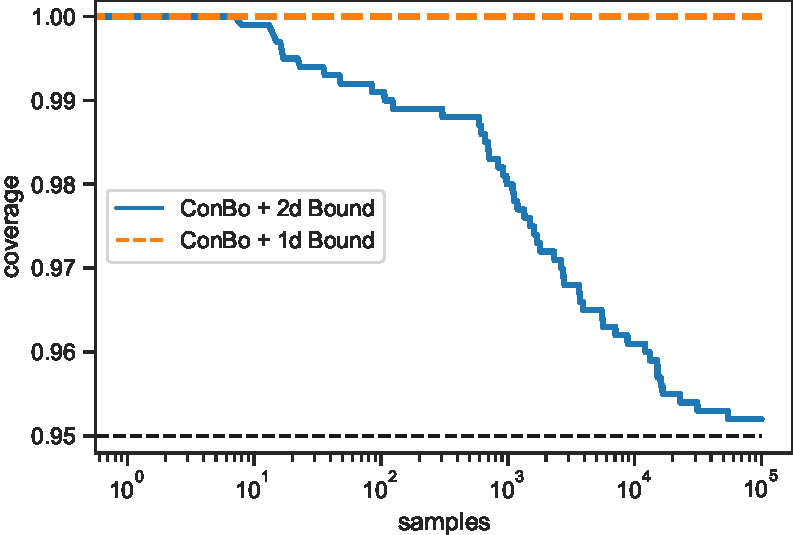
\includegraphics[width=0.75\linewidth]{coverage}
    \caption{Empirical coverage for two proposed CSs. The CS that bets on 
    both $w-1$ and $wr-v$ converges to nominal coverage while the CS
    that does not bet on $w-1$ overcovers.}
    \label{fig:coverage}
\end{figure}

\begin{table}
\caption{Timings for MOPE and its ablations on 500000 samples}
\label{tab:timings}
\centering
\begin{small}
\begin{sc}
\begin{tabular}{lcccr}
\toprule
Method & MOPE & $-$Vector & $-$Common & $-$Bound \\
\midrule
Time (sec)& 32     & 14.5  & 10440 & 15882 \\
\bottomrule
\end{tabular}
\end{sc}
\end{small}
\end{table}

\begin{figure*}
    \centering
    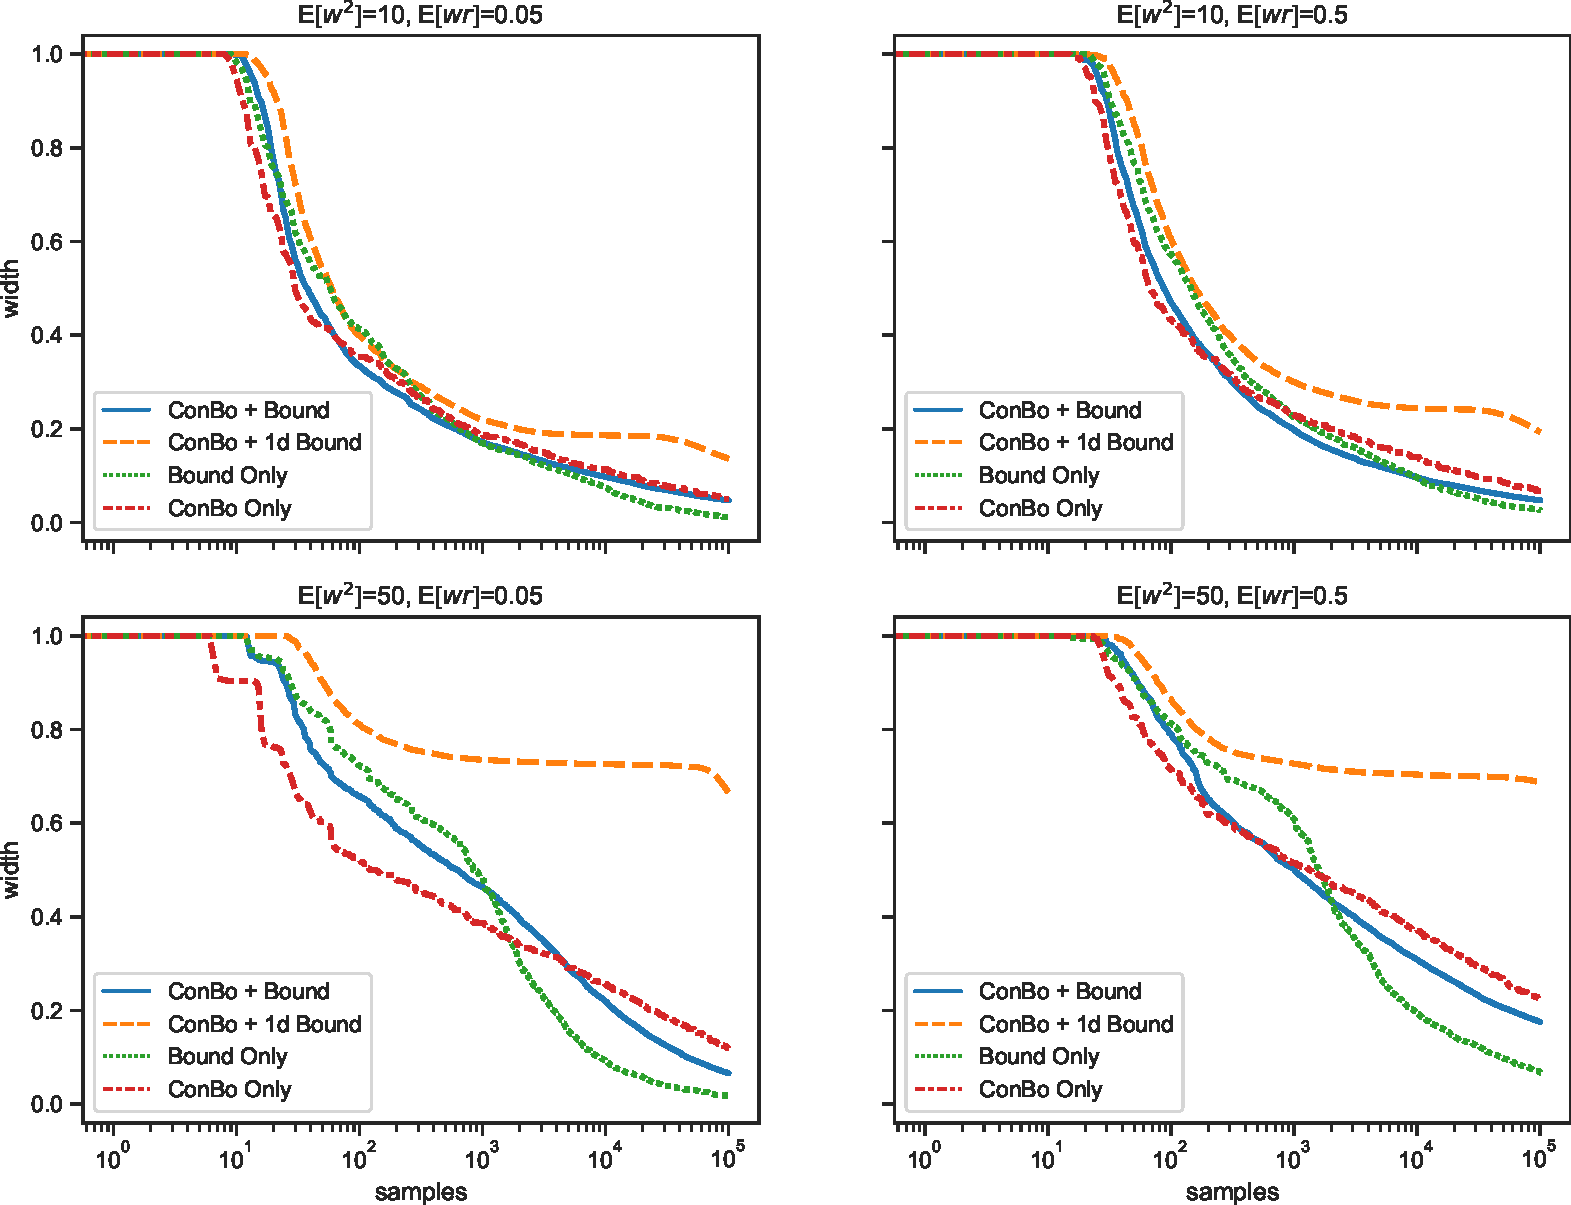
\includegraphics[width=0.8\textwidth]{width}
    \caption{The width of 95\% CS produced by MOPE and its three ablations.
    The pointwise asymptotic curve is \emph{not} a CS.}
    \label{fig:width}
\end{figure*}

\begin{figure}
    \centering
    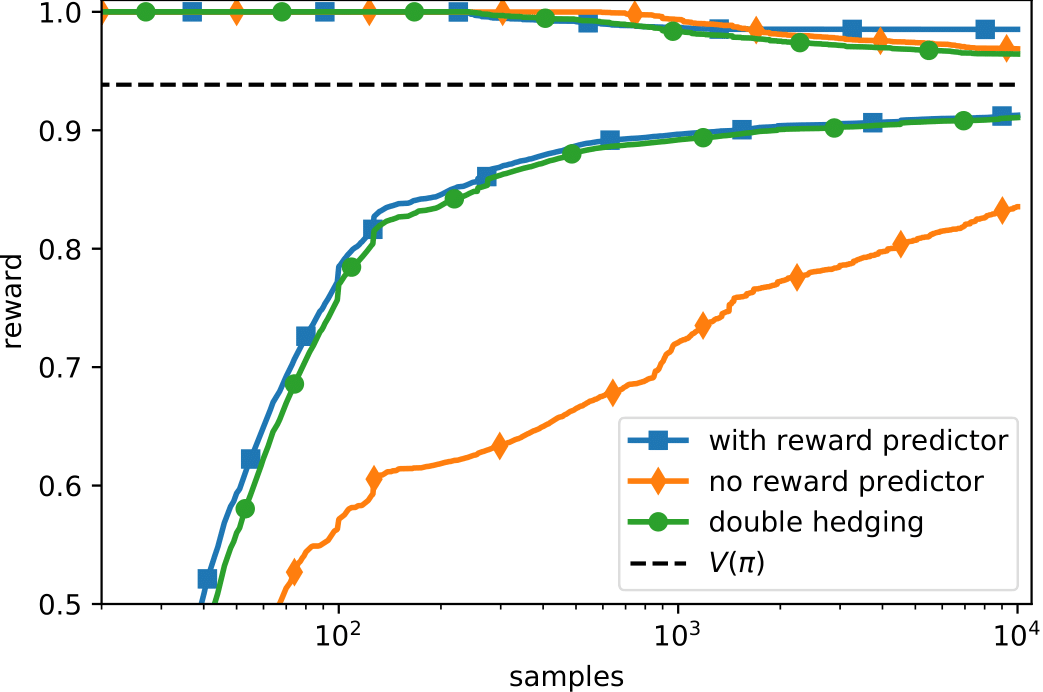
\includegraphics[width=0.75\linewidth]{predictor}
    \caption{Two 99.9\% CSs with and without a reward predictor.}
    \label{fig:predictor}
\end{figure}

\begin{figure}
    \centering
    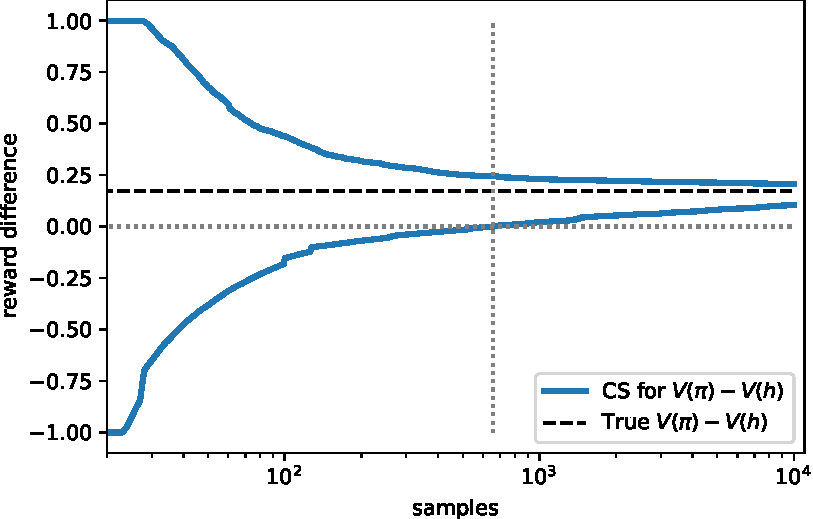
\includegraphics[width=0.75\linewidth]{gd}
    \caption{CS for the gated deployment experiment. $\pi$ can be 
    deployed as soon as the lower CS crosses 0 (dotted line, $t=657$)}
    \label{fig:gd}
\end{figure}

\subsection{Coverage} \label{sec:coverage}
While any predictable betting sequence
guarantees correct coverage, some will overcover more than
others. Here we investigate the coverage properties of
MOPE and the strategy of Section~\ref{sec:scalar}.
We generate 1000 sequences of 100000 $(w,r)$ pairs each from a different
distribution. All distributions are maximum entropy distributions subject to
$(w,r) \in \{0, 0.5, 2, 100\} \times \{0,1\}$, $\E[w]=1$, $\E[w^2]=10$
and $V(\pi)$ sampled uniformly in $[0,1]$. In Figure~\ref{fig:coverage} we show
the empirical mean coverage of the two CSs for $\alpha=0.05$. 
MOPE approaches nominal coverage from above,
a property rarely seen with standard confidence bounds.

\subsection{Computational vs. Statistical Efficiency}
We run an ablation study for the three ingredients of MOPE:
betting with a vector $\lambda$ (V)
optimizing a bound on wealth (B), 
and using common bets (C) for all $v$. We use 
the strategy of Section~\ref{sec:scalar} to study
the effect of (V). The alternative to (B) is to 
solve \eqref{eq:ftl} instead of \eqref{eq:quadopt} in
Algorithm~\ref{alg:main}.
The alternative to (C) is to maintain a 
grid of $v$ values and solve
\eqref{eq:quadoptv} for each element of the grid
at each timestep. We use four synthetic environments
which are distributions over $(w,r)$ generated in the same way as section~\ref{sec:coverage} but
with $(V(\pi),\E[w^2]) \in \{0.05, 0.5\} \times \{10, 100\}$.

Table~\ref{tab:timings}
shows the running times for each method in the environment with 
the largest variance. We see that directly 
maximizing wealth and individual betting per $v$ are very slow.
MOPE and the scalar betting strategy are computationally efficient.
In Figure~\ref{fig:width} we show the 
average CS width over 10 repetitions for 500000 time steps
for MOPE and its ablations as well as the 
asymptotic confidence interval from~\cite{karampatziakis2019empirical}
which is only valid \emph{pointwise} and provides a lower bound for
all CSs in the figure. While MOPE is not as tight as
the (much slower) individual bet ablation the gap is small in all 
but the most challenging environment.

\subsection{Effect of a Reward Predictor}
We now investigate whether the availability of a good 
reward predictor can tighten our CS using the process
$K_t^{\pm q}(v)$ of Section~\ref{sec:reward-predictor}.
We use the first 1 million samples from the mnist8m
dataset which has 10 classes and train the following
functions: $h$ using linear multinomial 
logistic regression (MLR), $\pi$ again using MLR but
now on $1000$ random Fourier 
features (RFF)~\cite{rahimi2007random} that approximate 
a Gaussian kernel machine, and finally $q$ which
uses the same RFF represetation as $\pi$ but instead
its $i$-th output is independently trained 
to predict whether the input is the $i$-th class
using 10 binary logistic regressions.
We used the rest of the data with the following 
protocol: for each input/label pair $(x_i,y_i)$, we sample 
action $a_i$ with probability $0.9h(a_i;x_i)+0.01$
(so that we can safely set $w_{\max}=100$),
we set $r_i=1$ if $a_i=y_i$, otherwise $r_i=0$, 
and record $w_i$ and $c_i$. We estimated 
$V(\pi)\approx 0.9385$ using the next million samples
and observed a 13x reduction in variance when using
$w_i r_i - c_i$ vs. $w_i r_i$. In Figure~\ref{fig:predictor}
we show the CS for $V(\pi)$ averaged over 5 runs each 
with 10000 different samples using the hedged processes 
$K_t^{\pm q}(v)$ and $K_t^{\pm}(v)$.
We see that including 
a reward predictor dramatically improves the lower bound
and somewhat hurts the upper bound. Why does the upper
bound become worse? In the hedged process the upper bound 
is computed via a lower bound with rewards equal to 
$1-r$. Because $\pi$ is a very good policy, $1-r$ is 
typically close to $0$. Since$K_t^{\pm}$ can be 
thought of as $K_t^{\pm}$ with a reward predictor of 0,
we expect it to work very well in this setup.

\subsection{Regret in Gated Deployment}
We take a dataset and use the first part to train $h$ in a 
bandit way and we also reward predictors. We use 
$h$ to collect data from the second part. We train
$\pi_1,\ldots, \pi_k$ on the second part. We run 
on the last part and measure regret against the
best $\pi$. 

\section{Conclusions}
We presented a generic way to construct confidence sets for OPE in the single
step CB setting. The construction leaves a lot of freedom in designing betting
sequences and we mostly explored options with an eye towards computational
efficiency. The generality of our approach makes us hopeful 

\bibliography{opecs}
\bibliographystyle{unsrtnat}
\newpage
\onecolumn
\appendix
\section{Proofs}

\subsection{Proof of Theorem~\ref{thm:martingale}}
\subsection{Proof of Theorem~\ref{thm:ville}}
\subsection{Proof of Theorem~\ref{thm:cs}}
\subsection{Proof of Lemma~\ref{lem:quadbound}}
\subsection{Proof of Theorem~\ref{thm:hedged}}
\section{Avoiding grid search}
\label{app:nogrid2d}
We first lower bound each process separately, then lower bound
the hedged process. We denote the bets for $K^{+}$ (respectively
$K^{-}$) as $\lambda^{+}$, (resp. $\lambda^{-}$).
From lemma~\ref{lem:quadbound} we have
\[
\ln(K_t^{+}(v)) \geq \sum_{i=1}^{t-1} {\lambda_i^{+}}^\top b_i(v) + \psi \sum_i {\lambda_i^{+}}^\top A_i(v) {\lambda_i^{+}}
\]
and
\[
\ln(K_t^{-}(v)) \geq \sum_{i=1}^{t-1} {\lambda_i^{-}}^\top b_i'(v') + \psi \sum_i {\lambda_i^{-}}^\top A_i'(v') {\lambda_i^{-}}
\]
where $v'=1-v$, 
$b_i'(v)=
\cvec{w_i-1}{w_i (1-r_i) -v}
$
and $A_i'(v)=b_i'(v)b_i'(v)^\top$.
For the Hedged process, using that for any $a,b$
\[
\ln\left(\exp(a)+\exp(b)\right)\geq \max(a,b)
\]
to first establish
\[
\ln(K^{\pm}(v)) \geq \max(\ln(K^{+}(v))-\ln(2),\ln(K^{-}(v))-\ln(2))
\]
and further bound each term in the maximum by the respective 
quadratic lower bound. We conclude that
if a $v$ achieves 
\[
 \sum_{i=1}^{t-1} {\lambda_i^{+}}^\top b_i(v) + \psi \sum_i {\lambda_i^{+}}^\top A_i(v) \lambda_i^{+} = \ln\left(\frac{2}{\alpha}\right)
\]
or a $v'=1-v$ achieves 
\[
\sum_{i=1}^{t-1} {\lambda_i^{-}}^\top b_i'(v') + \psi \sum_i {\lambda_i^{-}}^\top A_i'(v') \lambda_i^{-} = \ln\left(\frac{2}{\alpha}\right)
\]
then we also achieve $K_t^{\pm}(v) \geq \frac{1}{\alpha}$.
In terms of $v$ and $v'$ these expressions are second degree
equations and thus their real roots in $[0,1]$ (if any) provide 
a safe bracketing of the confidence region $\{v:K_t^{\pm}(v)\leq 1/\alpha\}$. For $K_t^{+}$ let
\begin{align}
C_t&= \sum_{i=1}^{t-1} {\lambda_i^{+}}^\top \cvec{w_i-1}{w_i r_i} \label{eq:upsuffc}\\
S_t&= \sum_{i=1}^{t-1} {\lambda_i^{+}}^\top \cvec{0}{1} \\
Q_t&= \sum_{i=1}^{t-1} \psi  {\lambda_i^{+}}^\top \symmat{(w_i-1)^2}{(w_i-1)w_i r_i}{w_i^2r_i^2} \lambda_i^{+} \\
T_t&= \sum_{i=1}^{t-1} \psi  {\lambda_i^{+}}^\top \symmat{0}{-(w_i-1)}{-2w_ir_i} \lambda_i^{+} \\
U_t&=  \sum_{i=1}^{t-1} \psi {\lambda_i^{+}}^\top \symmat{0}{0}{1} \lambda_i^{+} \label{eq:upsuffu}
\end{align}
and define $C_t',S_t',Q_t',T_t',U_t'$ similarly by using $\lambda_i^{-}$ 
instead of $\lambda_i^{+}$ and $1-r_i$ instead of $r_i$. Then
the largest real root $v^{+}$ of
\[
C_t - S_t v + Q_t + T_t v + U_t v^2 - \ln\left(\frac{2}{\alpha}\right) = 0,
\]
if it exists, satisfies $K_t^{\pm}(v^{+})\geq \frac{1}{\alpha}$. Similarly
we can obtain $v'$ as the largest real root of the quadratic
with $C_t',S_t',Q_t',T_t',U_t'$ in place of $C_t,S_t,Q_t,T_t,U_t$,
if it exists. Then $v^{-}=1-v'$ satisfies $K_t^{\pm}(v^{-})\geq \frac{1}{\alpha}$.



\section{Details of our Scalar Betting Strategy}
\subsection{Elimination of one bet} \label{app:betaopt}
Since the $\lambda_1$ bet cannot provide any long-term benefit, its purpose can only be as a hedge in the short-term. 
We formulate this by considering the
worst case wealth reduction among three outcomes :
$(w,r)=(w_{\max},1)$, 
$(w,r)=(w_{\max},0)$ and $w=0$ with any reward. 
We choose $\lambda_1$ to maximize the wealth 
in the worst of these outcomes. Thus we set 
up a family of Linear Programs (LPs) 
parametrized by $\lambda_2$ and $v$ and with optimization variables $\alpha$ and $\lambda_1$:
\begin{equation*}
\begin{array}{ll@{}ll}
\text{maximize}  & \alpha &\\
\text{subject to}& \alpha \leq 1+\lambda_1(w_{\max}-1)+\lambda_2(w_{\max}-v)  & &(z_1) \\
                 & \alpha \leq 1+\lambda_1(w_{\max}-1)-\lambda_2 v            & &(z_2) \\
                 & \alpha \leq 1-\lambda_1-\lambda_2 v                        & &(z_3) \\
\end{array}
\end{equation*}
Where the variable $z_i$ in parentheses next to each constraint is the corresponding dual variable. 
\begin{theorem}
For any $v\in [0,1]$ and any $\lambda_2 \in \R$, the optimal value of $\lambda_1$ in the above LP is $\lambda_1^*=\max(-\lambda_2,0)$.
\end{theorem}
\begin{proof}
The dual program is
\begin{equation*}
\begin{array}{ll@{}ll}
\text{minimize}  & (1+\lambda_2(w_{\max}-v))z_1 +(1-\lambda_2 v) z_2 + (1-\lambda_2 v) z_3 &\\
\text{subject to}& z_i \geq 0  & i=1,2,3 \\
                 & -(w_{\max}-1)(z_1+z_2)+z_3 = 0 \\
                 & z_1+z_2+z_3=1 \\
\end{array}
\end{equation*}
Consider the following two dual feasible settings:
\[
z_1=0,z_2=\frac{1}{w_{\max}}, z_3=\frac{w_{\max}-1}{w_{\max}}
\]
and 
\[
z_1=\frac{1}{w_{\max}}, z_2=0, z_3=\frac{w_{\max}-1}{w_{\max}}
\]
with corresponding dual objectives: $1-\lambda_2 v$ and $1-\lambda_2 v + \lambda_2$. From here we see that if $\lambda_2 > 0$ the former attains a
better dual objective and is thus a better bound
for the primal objective. When $\lambda_2<0$ the latter
is better. 

When $\lambda_2>0$, a primal feasible setting is
$\alpha=1-\lambda_2 v,\lambda_1=0$. Furthermore this setting
achieves the same objective as the first dual feasible setting so 
we conclude that these are the optimal primal and dual solutions when $\lambda_2>0$.

When $\lambda_2<0$, a primal feasible setting is 
$\alpha=1-\lambda_2 v +\lambda_2, \lambda_1=-\lambda_2$. Furthermore this setting
achieves the same objective as the second dual feasible setting
so we conclude that these are the optimal primal and dual solutions when $\lambda_2<0$. 

Finally when $\lambda_2=0$ the two cases give the same value for $\lambda_1$ so we conclude $\lambda_1=\max(-\lambda_2,0)$ for all $\lambda_2 \in \R$ (and $v\geq 0$).
\end{proof}

\subsection{A Technical Lemma}
\label{app:fan}
The following result can be extracted from the proof of 
Proposition~4.1 in \cite{fan2015exponential}.
\begin{lemma}
For $\xi\geq -1$ and $\lambda \in [0,1)$ we have
\begin{equation}
\ln(1+\lambda \xi) \geq \lambda \xi+\left(\ln\left(1-\lambda\right)+\lambda\right)\cdot \xi^{2}
\label{eq:fanbound}
\end{equation}
\end{lemma}
\begin{proof}
Note that $\lambda \xi \geq -\lambda > -1$. 
For $x>-1$ the function $f(x) = \frac{\ln(1 + x)-x}{x^2}$
is increasing in $x$, therefore
$f(\lambda \xi) \geq f(-\lambda)$. Rearranging
leads to the statement of the lemma.
\end{proof}
We will be using this lemma with bets 
$\lambda \in [0,1)$ and $\xi_i=w_ir_i-v$ or $\xi_i=w_i(1-r_i)-(1-v_i)$.
In either case $\xi_i\geq -1$.
This lemma provides a stronger lower bound than 
that of Lemma~\ref{lem:quadbound}. The reason
we use the latter for vector bets is that the
natural extension of \eqref{eq:fanbound} to 
the vector case does not lead to a convex 
problem. 

\subsection{Avoiding grid Search}
\label{app:nogrid1d}
Suppose that our bets $\lambda_{2,i}^{+}$ and $\lambda_{2,i}^{-}$ 
do not depend on $v$.
We have the individual lower bounds
\[
\ln(K^{+}(v)) \geq \sum_i \lambda_{2,i}^{+} (w_i r_i -v) + \sum_i (\ln(1-\lambda_{2,i}^{+})+\lambda_{2,i})(w_i r_i -v)^2
\]
and
\[
\ln(K^{-}(v)) \geq \sum_i \lambda_{2,i}^{-} (w_i r_i' -v') + \sum_i (\ln(1-\lambda_{2,i}^{-})+\lambda_{2,i}^{-})(w_i r_i' -v')^2
\]
where $r'=1-r$, $v'=1-v$.
For the Hedged process, using that for any $a,b$
\[
\ln\left(\exp(a)+\exp(b)\right)\geq \max(a,b)
\]
to first establish
\[
\ln(K^{\pm}(v)) \geq \max(\ln(K^{+}(v))-\ln(2),\ln(K^{-}(v))-\ln(2))
\]
and further bound each term in the maximum by the respective 
quadratic lower bound. We conclude that
if a $v$ achieves 
\[
\sum_i \lambda_{2,i}^{+} (w_i r_i -v) + \sum_i (\ln(1-\lambda_{2,i}^{+})+\lambda_{2,i}^{+})(w_i r_i -v)^2 = \ln\left(\frac{2}{\alpha}\right)
\]
or a $v'=1-v$ achieves 
\[
\sum_i \lambda_{2,i}^{-} (w_i r_i'-v') + \sum_i (\ln(1-\lambda_{2,i}^{-})+\lambda_{2,i}^{-})(w_i r_i' - v')^2
=\ln\left(\frac{2}{\alpha}\right)
\]
then we also achieve $K^{\pm}(v) > \frac{1}{\alpha}$. 
Thus, a valid confidence interval can be obtained by considering
the roots of these quadratics.  Let
\begin{align*}
C&=\sum_i \lambda_{2,i}^{+} w_i r_i & 
C'&=\sum_i \lambda_{2,i}^{-} w_i r_i'\\
S&=\sum_i \lambda_{2,i}^{+} & 
S'&=\sum_i \lambda_{2,i}^{-} \\
Q&=\sum_i \left(\ln(1-\lambda_{2,i}^{+})+\lambda_{2,i}^{+}\right) w_i^2 r_i^2 &
Q'&=\sum_i \left(\ln(1-\lambda_{2,i}^{-})+\lambda_{2,i}^{-}\right) w_i^2 r_i'^2\\
T&=\sum_i \left(\ln(1-\lambda_{2,i}^{+})+\lambda_{2,i}^{+}\right) w_ir_i &
T'&=\sum_i \left(\ln(1-\lambda_{2,i}^{-})+\lambda_{2,i}^{-}\right) w_ir_i'\\
U&=\sum_i \left(\ln(1-\lambda_{2,i}^{+})+\lambda_{2,i}^{+}\right) &
U'&=\sum_i \left(\ln(1-\lambda_{2,i}^{-})+\lambda_{2,i}^{-}\right)\\
\end{align*}
We obtain:
\[
v_{\min}= \frac{2T+S-\sqrt{(2T+S)^2-4U(Q+C-\ln(2/\alpha))}}{2U}
\]
or $v_{\min}=0$ if the discriminant is negative, 
and
\[
v_{\max}=1-v' = 1-\frac{2T'+S'-\sqrt{(2T'+S')^2-4U'(Q'+C'-\ln(2/\alpha))}}{2U'}
\]
or $v_{\max}=1$ if the discriminant is negative.

\section{Reward Predictors}
\label{app:reward-predictors}
Given a measurable reward predictor $q(x,a)$ 
with codomain $[0,1]$ we define
$
c_i = w_i q(x_i,a_i) - \sum_{a'} \pi(a';x_i)q(x_i,a')
$ 
with $\E[c_i]=0$ and $-1\leq c_i \leq w_{\max}-1$.

\subsection{Wealth Lower Bound}
We 
We overload the log wealth at step $i$ when betting against $v$ as 
$\ell_i^v(\lambda) = \ln(1+\lambda_{0,i} c_i + \lambda_{1,i}(w_i-1) + \lambda_{2,i}(w_i r_i -v)$
We use Lemma~\ref{lem:quadbound} to obtain
\[
\sum_{i=1}^{t-1} \ell_i^v(\lambda) \geq \lambda^\top \sum_{u=1}^{t} 
\]

We distinguish between linear and nonlinear reward predictors.
A reward predictor is a function $f(x,a)$ mapping
context and action to estimated reward. A linear 
reward predictor can be written
as $f(x,a)=\theta^\top z(x,a)$ for some vector of parameters
$\theta$ and a vector of features $z(x,a)$, while a 
nonlinear reward predictor cannot. 

Let
\[
G(f,w,x,a)= w f(x,a) - \sum_{a'} \pi(a';x) f(x,a')
\]
In both cases we leverage that for a predictable $f$
\[
\E_{x\sim D,a\sim h(x)}\left[G(f,w,x,a)\right] = 0
\]
Note that $\E[w]=1$ is a special case of the above 
for the constant function $f(x,a)=1$. 

For a nonlinear reward predictor we define the capital 
process as
\[
K(v)=\prod_{i} \left(1+\lambda_{1,i} (w_i -1) 
+ \lambda_{2,i} (w_i r_i -v) 
+ \lambda_{3,i} G(f,w_i,x_i,a_i)\right)
\]
we can then proceed as before but with one additional
bet.

For a linear reward predictor we can do the same
as above or alternatively we can absorb the 
parameters in the bets:
\[
K(v)=\prod_{i} \left(1+\lambda_{1,i} (w_i -1) 
+ \lambda_{2,i} (w_i r_i -v) 
+ \lambda_{3,i} G(\theta_i^\top z, w_i,x_i,a_i)\right)
\]
\[
=\prod_{i} \left(1+\lambda_{1,i} (w_i -1) 
+ \lambda_{2,i} (w_i r_i -v) 
+ \nu_i^\top \left(w_i z(x_i,a_i) - \sum_{a'} \pi(a';x_i) z(x_i,a') \right)\right)
\]
where $\nu_i = \lambda_{3,i}\theta_i$ is a new vector bet.

This construction can be used with a time varying $z$
such as the last layer of a neural net. However, the algorithms
we have proposed are assuming iid data (in particular FTL schemes
can have linear regret in the non-iid case) and so one would need to use online algorithms to safely increase the wealth.
